
\part[Algoritmos sequenciais, condicionais e com repetições]
{Algoritmos sequenciais, condicionais e com repetições}


\chapter[Algoritmos sequenciais]
{Algoritmos sequenciais}


\section*{Resumo}

Estrutura sequencial é um conjunto de instruções que serão executadas em sequência. A sequência de cada instrução deve ser seguida apara a realização de uma tarefa.

\section*{Pré-requisitos}

As práticas deste capítulo exigem que sejam utilizadas as funções
\begin{itemize}
  \item 
    \begin{lstlisting}[language=C++]
    void AbreJanela(float largura, float altura, const char* titulo)
    \end{lstlisting}

  \item
    \begin{lstlisting}[language=C++]
    void PintaFundo(int red, int green, int blue)
    \end{lstlisting}

  \item
    \begin{lstlisting}[language=C++]
    void MostraPlanoCartesiano ( int intervalo )
    \end{lstlisting}

  \item
    \begin{lstlisting}[language=C++]
    void Desenha()
    \end{lstlisting}

  \item
    \begin{lstlisting}[language=C++]
    void Pintar ( int red , int green , int blue )
    \end{lstlisting}

  \item
    \begin{lstlisting}[language=C++]
    int CriaCirculo ( float raio , Ponto meio)
    \end{lstlisting}

    \item
    \begin{lstlisting}[language=C++]
    int CriaElipse ( float a , float b, Ponto meio)
    \end{lstlisting}

    \item
    \begin{lstlisting}[language=C++]
    int CriaQuadrado( float lado , Ponto cantoesq )
    \end{lstlisting}

    \item
    \begin{lstlisting}[language=C++]
    int CriaRetangulo ( float base , float altura , Ponto cantoesq )
    \end{lstlisting}

    \item
    \begin{lstlisting}[language=C++]
    int CriaTriangulo ( float base , float altura , Ponto cantoesq )
    \end{lstlisting}

    \item
    \begin{lstlisting}[language=C++]
    int CriaPoligono ( short int qtd , . . . )
    \end{lstlisting}
\end{itemize}

%\begin{chapreferences}{1.}
%\bibliography{playAPC{}}
%\bibliographystyle{plain}
%\nocite{cbook}
%\nocite{sb6}
%\nocite{glfw}
%\nocite{cppbook}

%\end{chapreferences}

% \begin{chapreferences}{1}

% \bibitem{sb6}
% {\em OpenGL SuperBible}.
% \newblock Pearson Education Inc, 6 edition, 2014.

% \bibitem{glfw}
% Marcus Geelnard and Camilla Berglund.
% \newblock {\em GLFW - Reference guide}, 2010.
% \newblock API version 2.7.

% \bibitem{cbook}
% Brian~W. Kernighan and Dennis~M. Ritchie.
% \newblock {\em The C Programming Language}.
% \newblock 1989.

% \bibitem{cppbook}
% Stanley~B. Lippman, Josés Lajoile, and Barbara Moo.
% \newblock {\em C++ Primer}.
% \newblock 2013.
% \end{chapreferences}

\section*{Problemas}
\begin{enumerate}
\item
  Exiba um plano cartesiano de -100 a 100 com espaçamento de 5 unidades.
  \label{ex:cap01_ex1}

  \begin{figure*}[!htb]
    \centering
    \begin{subfigure}[b]{0.3\textwidth}
        \centerline{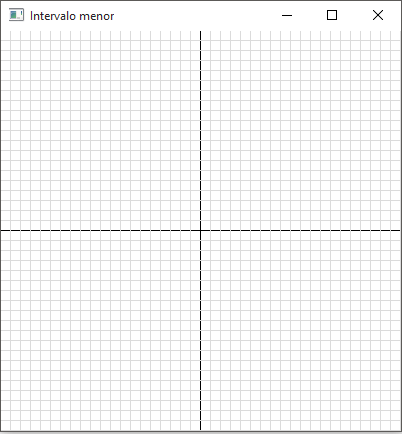
\includegraphics[width=.9\textwidth]{img/cap1_ex1.png}}
        \caption{Visualização de todo plano cartesiano}
        \label{fig:cap01_ex1}
    \end{subfigure}
    ~
    \begin{subfigure}[b]{0.65\textwidth}
        \centerline{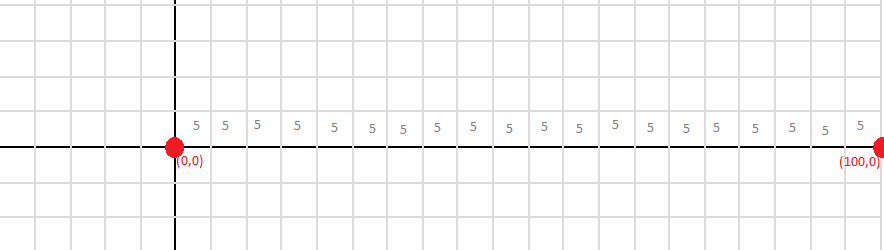
\includegraphics[width=.9\textwidth]{img/cap1_ex1_b.png}}
        \caption{De (0,0) até (100,0), existem 20 quadrados com 5 unidades de tamanho}
        \label{fig:cap01_ex1}
    \end{subfigure}
    \caption{Plano cartesiano de -100 à 100}
\end{figure*}


\item
  Desenhe um boneco palito que utilize pelo menos uma vez as seguintes geometrias:
  \begin{itemize}
  \item
    Círculo
  \item
    Elipse
  \item
    Retângulo
  \item
    Triângulo
  \item
    Quadrado
  \end{itemize}
  \label{ex:cap01_ex2}

  \begin{figure}[H]
    \centerline{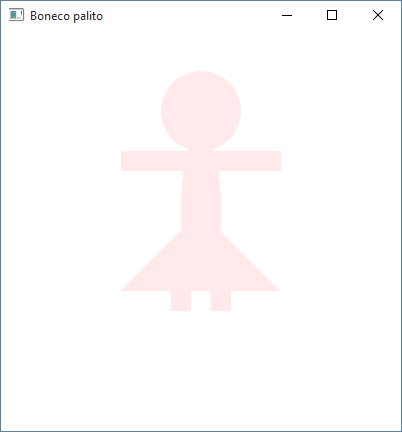
\includegraphics[width=.5\textwidth]{img/cap1_ex3.png}}
    \caption{Boneco Palito}
    \label{fig:cap01_ex2}
  \end{figure}

\item
  Exiba a estrela de Davi.
  \label{ex:cap01_ex3}

  \begin{figure}[H]
    \centerline{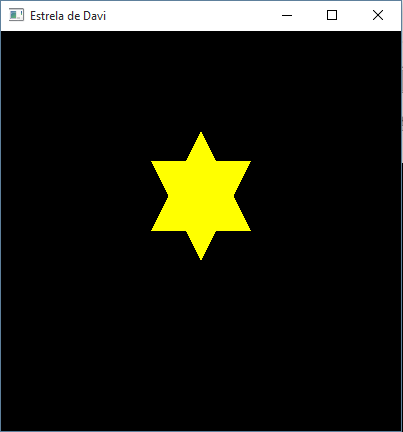
\includegraphics[width=.5\textwidth]{img/cap1_ex2.png}}
    \caption{Estrela de Davi}
    \label{fig:cap01_ex3}
  \end{figure}

  \item
  Escreva um programa que solicite do usuário um raio de um círculo e exiba um quadrado inscrito neste círculo.
  \label{ex:cap01_ex8}

  \begin{figure}[H]
    \centerline{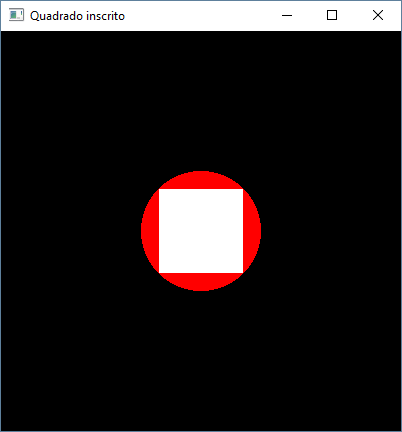
\includegraphics[width=.5\textwidth]{img/cap1_ex21}}
    \caption{Quadrado inscrito em um círculo}
    \label{fig:cap01_ex8}
  \end{figure}

\end{enumerate}


\section*{Soluções}

\subsection*{Exercício \ref{ex:cap01_ex1}}

Esta prática se refere a exibir um Plano Cartesiano na tela com espaçamento de 5 em 5 unidades, tanto no eixo x quanto no eixo y. Com ela, o aluno poderá notar a importância da ordem de chamada de funções da \playAPC{} e a necessidade das funções \emph{AbreJanela} e \emph{Desenha}, além de verificar, com um exemplo simples, se a playAPC{} foi corretamente bem instalada.

\lstinputlisting[caption=Código fonte de Plano Cartesiano, style=customc, label=lst:cap1_ex1]{src/ex1_PrimeiraJanela.cpp}

\begin{lstlisting}[label={func:AbreJanela},language=C++]
void AbreJanela(float largura, float altura, const char* titulo)
\end{lstlisting}

A função \emph{AbreJanela}, na linha \ref{line:AbreJanela}, inicializa todas as variáveis utilizadas pela biblioteca, e preferencialmente é a chamada antes de qualquer outra função da \playAPC{}. Por padrão, o plano de renderização está limitado de (-100,100) em coordenadas $x,y$ do plano cartesiano. Este valor pode ser alterado utilizando a função \emph{MostraPlanoCartesiano} antes de chamar \emph{AbreJanela}.
Seu primeiro argumento se refere a largura da janela, o segundo a altura, sendo ambos do tipo inteiro, e o terceiro se refere ao nome que a janela terá, sendo uma string.


\begin{lstlisting}[label={func:PintarFundo},language=C++]
void PintaFundo(int red, int green, int blue)
\end{lstlisting}
A função \emph{PintarFundo}, na linha \ref{line:PintarFundo}, é específica para pintar o fundo da janela de contexto aberto pela função \emph{AbreJanela}. Seu argumentos utiliza o sistema de cores \emph{RGB} (\emph{red}, \emph{green}, \emph{blue}), utilizando a escala de 0 até 255.

\begin{lstlisting}[label={func:MostraPlanoCartesiano},language=C++]
void MostraPlanoCartesiano(int intervalo)
\end{lstlisting}
A função \emph{MostraPlanoCartesiano}, na linha \ref{line:MostraPlanoCartesiano} exibe o plano de coodernadas cartesianas, plano utilizado para o posicionamento das geometrias criadas pela \playAPC{}. Como as unidades no plano cartesiano não se referem ao posicionamento direto do pixel, a exibição do plano cartesiano com esta função serve de auxílio para o usuário posicionar suas geometrias na janela sem se preocupar com redimensionamento ou posição que a janela se encontra na tela do usuário. Para $x = 0$ e $y = 0$, as retas são pretas e as demais são cinza.
Seu único argumento se refere de quantas em quantas unidades do plano terão uma reta vertical e horizontal da cor cinza.

\begin{lstlisting}[label={func:Desenha},language=C++]
void Desenha()
\end{lstlisting}
A função \emph{Desenha}, na linha \ref{line:Desenha}, realiza o loop de renderização. Todas as geometrias criadas até esta chamada de função serão renderizadas e permanecerão estáticas, não havendo a possibilidade de posteriores animações.
Para encerrar o loop de renderização, basta fechar a janela clicando no botão de fechar ou apertando a tela \emph{ESC}. Após fechar a janela, todo o contexto da \playAPC{} será encerrado e as áreas de memórias alocadas serão liberadas.

\subsection*{Exercício \ref{ex:cap01_ex2}}

Esta prática se refere a exibir um boneco palito e praticar a grande maioria das geometrias pré-definidas existentes na \playAPC{}. Os argumentos de cada função podem ser consultados no Guia de Referência da playAPC{} \footnote{\url{http://playapc.zaghetto.com/category/funcoes/geometrias}}
\lstinputlisting[caption=Código fonte do boneco palito, style=customc, label=lst:cap1_ex2]{src/ex3_boneco.cpp}

\begin{lstlisting}[label={func:Ponto},language=C++]
struct Ponto{
    float x;
    float y;
}
\end{lstlisting}
Ponto, na linha \ref{line:estruturaPonto}, é uma estrutura do tipo float com dois membros, \emph{x} e \emph{y}, os quais devem ser utilizados como coordenadas do plano cartesiano 2D. Esta estrutura possui sobrecarga para os seguintes operadores =, +, -, +=, -=, == e !=.
\begin{itemize}
  \item =
    \begin{lstlisting}[style=customc,language=C++]
    Ponto p1, p2;
    (...)

    p1 = p2;
    \end{lstlisting}
   \item + (ou -)
    \begin{lstlisting}[style=customc,language=C++]
    Ponto p1, p2, p3;
    (...)

    p1 = p2 + p3;
    \end{lstlisting} 
     \item += (ou -=)
    \begin{lstlisting}[style=customc,language=C++]
    Ponto p1, p2;
    (...)

    p1 += p2;
    \end{lstlisting}

     \item == (ou !=)
    \begin{lstlisting}[style=customc,language=C++]
    Ponto p1, p2;
    (...)

    if(p1 == p2){
      (...)
    }
    \end{lstlisting}
\end{itemize}

\begin{lstlisting}[label={func:Pintarm1},language=C++]
void Pintar(int red, int green, int blue); 
void Pintar(int red, int green, int blue, geometrias_validas nome, int index);
\end{lstlisting}
A função \emph{Pintar}, na linha \ref{line:Pintarm1} pode ser utilizada de duas formas. No caso da Listagem \ref{lst:cap1_ex2}, a última geometria criada receberá a cor definida por esta função, utilizando o sistema de cores RGB. A segunda forma de utilizar esta função está ilustrada na Listagem \ref{lst:cap2_ex2}.

\begin{lstlisting}[label={func:CriaCirculo},language=C++]
int CriaCirculo(float raio, Ponto meio)
\end{lstlisting}
A função \emph{CriaCirculo}, na linha \ref{line:CriaCirculo}, cria uma geometria do tipo \emph{CIRCULO}, retornando um índice deste tipo de geometria. Seu primeiro argumento é o tamanho do raio e o segundo argumento é onde estará centrado o círculo.

\begin{lstlisting}[label={func:CriaElipse},language=C++]
int CriaElipse(float a, float b, Ponto meio)
\end{lstlisting}
A função \emph{CriaElipse}, na linha \ref{line:CriaElipse}, cria uma geometria do tipo \emph{ELIPSE}, retornando um índice deste tipo de geometria. Seu primeiro argumento é a metade do maior eixo da elipse, o segundo é a metade do menor eixo da elipse e o terceiro argumento se refere onde a elipse estará centrada.

\begin{lstlisting}[label={func:CriaQuadrado},language=C++]
int CriaQuadrado(float lado, Ponto cantoesq)
\end{lstlisting}
A função \emph{CriaQuadrado}, na linha \ref{line:CriaQuadrado}, cria uma geometria do tipo \emph{QUADRADO}, retornando um índice deste tipo de geometria. Seu primeiro argumento é o tamanho do lado do quadrado e o segundo argumento é onde ficará localizado o ponto esquerdo inferior da geometria

\begin{lstlisting}[label={func:CriaRetangulo},language=C++]
int CriaRetangulo(float base, float altura, Ponto cantoesq)
\end{lstlisting}
A função \emph{CriaRetangulo}, na linha \ref{line:CriaRetangulo}, cria uma geometria do tipo \emph{RETANGULO}, retornando um índice deste tipo de geometria. Seu primeiro argumento é a base do retângulo, o segundo a altura não-negativa dele e o último é onde ficará localizado o ponto esquerdo inferior da geometria

\begin{lstlisting}[label={func:CriaTriangulo},language=C++]
int CriaTriangulo(float base, float altura, Ponto cantoesq)
\end{lstlisting}
A função \emph{CriaTriangulo}, na linha \ref{line:CriaTriangulo}, cria uma geometria do tipo \emph{TRIANGULO}, retornando um índice deste tipo de geometria. Seu primeiro argumento é a base do triângulo, o segundo a altura não-negativa dele e o último é onde ficará localizado o ponto esquerdo inferior da geometria

\subsection*{Exercício \ref{ex:cap01_ex3}}

Esta prática se refere a exibir a estrela de Davi, feita com dois triângulos. Um triângulo foi criado com a função \emph{CriaTriangulo} e o outro com a função \emph{CriaPoligono}. Verificamos nesta prática os argumentos de \emph{CriaTriangulo} (base, altura e ponto esquerdo inferior) e, como não há como ter altura negativa, teve a necessidade de criar um polígono definido pelos três pontos \emph{p1, p2} e \emph{p3} para criar-se um triângulo \emph{de cabeça pra baixo}.
\lstinputlisting[caption=Código fonte da Estrela de Davi, style=customc, label=lst:cap1_ex3]{src/ex2_davi.cpp}

\begin{lstlisting}[label={func:CriaPoligono},language=C++]
int CriaPoligono(short int qtd, ...)
\end{lstlisting}
A função \emph{CriaPoligono}, na linha \ref{line:CriaPoligono}, cria uma geometria do tipo \emph{POLIGONO}, retornando um índice deste tipo de geometria. Seu primeiro argumento é a quantidade de pontos que serão passados para esta função, e os seguintes argumentos serão os pontos propriamente ditos. Note que a \playAPC{} é limitada no aspecto que esta função só consegue renderizar figuras convexas. Caso haja a necessidade de criação de figuras não-convexas, será necessário \emph{"quebrar"} a geometria não-convexa em duas ou mais geometrias convexas.

\subsection*{Exercício \ref{ex:cap01_ex8}}

Esta prática se refere a exibir um quadrado inscrito em um círculo, a qual exercita o raciocínio matemático do aluno. O quadrado, criado pela função \emph{CriaQuadrado}, precisa de um ponto de referência para ser criado, sendo este ponto o inferior esquerdo. Desta forma, o aluno teria que calcular, dado o raio do círculo, não apenas o lado do quadrado, mas também a posição que este ponto de referência precisa estar.

\lstinputlisting[caption=Código fonte do quadrado inscrito, style=customc, label=lst:cap1_ex8]{src/ex21_inscrito.cpp}


\chapter[Algoritmos condicionais]
{Algoritmos condicionais}



\section*{Resumo}

Estrutura condicional expõe que a instrução ou bloco de instrução só seja executada se a condição for verdadeira.

\section*{Pré-requisitos}

As práticas deste capítulo exigem que sejam utilizadas as funções
\begin{itemize}
  \item 
    \begin{lstlisting}[language=C++]
    int CriaReta(Ponto p1 , Ponto p2)
    \end{lstlisting}

  \item
    \begin{lstlisting}[language=C++]
    void CriaPonto(Ponto p)
    \end{lstlisting}

  \item
    \begin{lstlisting}[language=C++]
    void Grafite(int espessura)
    \end{lstlisting}
 
\end{itemize}


%\begin{chapreferences}{1.}
%\bibliography{playAPC{}}
%\bibliographystyle{plain}
%\nocite{cbook}
%\nocite{sb6}
%\nocite{glfw}
%\nocite{cppbook}

%\end{chapreferences}

% \begin{chapreferences}{1}

% \bibitem{sb6}
% {\em OpenGL SuperBible}.
% \newblock Pearson Education Inc, 6 edition, 2014.

% \bibitem{glfw}
% Marcus Geelnard and Camilla Berglund.
% \newblock {\em GLFW - Reference guide}, 2010.
% \newblock API version 2.7.

% \bibitem{cbook}
% Brian~W. Kernighan and Dennis~M. Ritchie.
% \newblock {\em The C Programming Language}.
% \newblock 1989.

% \bibitem{cppbook}
% Stanley~B. Lippman, Josés Lajoile, and Barbara Moo.
% \newblock {\em C++ Primer}.
% \newblock 2013.
% \end{chapreferences}

\section*{Problemas}
\begin{enumerate}

\item
   Escreva um programa que solicita do usuário um raio, a posição do centro de uma circunferência e a posição de um ponto qualquer. Exiba a cena e indique no título da janela se o ponto está dentro ou fora da circunferência.

   \begin{figure*}[!htb]
    \centering
    \begin{subfigure}[b]{0.4\textwidth}
        \centerline{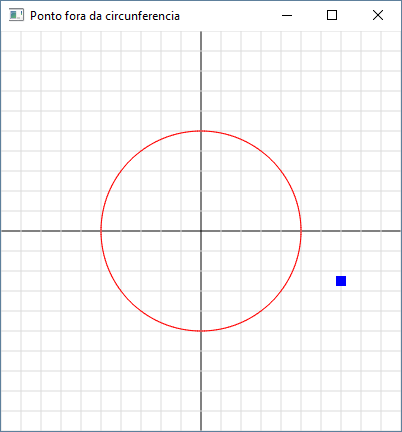
\includegraphics[width=.9\textwidth]{img/cap1_ex22}}
        \caption{Ponto está fora da circunferência}
        \label{fig:cap01_ex22a}
    \end{subfigure}
    ~
    \begin{subfigure}[b]{0.4\textwidth}
        \centerline{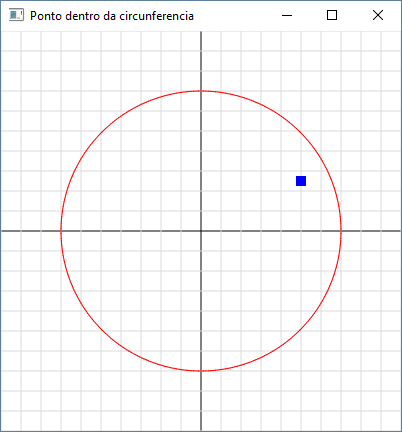
\includegraphics[width=.9\textwidth]{img/cap1_ex22b}}
        \caption{Ponto está dentro da circunferência}
        \label{fig:cap01_ex22b}
    \end{subfigure}

  \end{figure*}

  \label{ex:cap01_ex22}

\item
  Escreva um programa que receba do usuário um valor de ângulo em graus e um valor de raio. Converta para radianos o ângulo e exiba uma reta com o raio fornecido pelo usuário e pinte-a de acordo com as seguintes regras:
    \begin{itemize}
    \item
    Se a reta pertencer ao \emph{primeiro} quadrante, pinte-a de vermelho
    \item
    Se a reta pertencer ao \emph{segundo} quadrante, pinte-a de verde
    \item
    Se a reta pertencer ao \emph{terceiro} quadrante, pinte-a de azul
    \item
    Se a reta pertencer ao \emph{quarto} quadrante, pinte-a de preto
    \end{itemize}
    \label{ex:cap01_ex4}

  \begin{figure*}[h!]
    \centering
    \begin{subfigure}{0.2\textwidth}
        \centerline{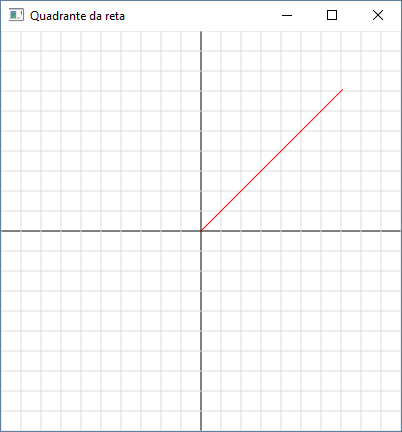
\includegraphics[width=.9\textwidth]{img/cap1_ex4}}
        \caption{Reta pertencente ao primeiro quadrante}
        \label{fig:cap01_ex4a}
    \end{subfigure}
    ~
    \begin{subfigure}{0.2\textwidth}
        \centerline{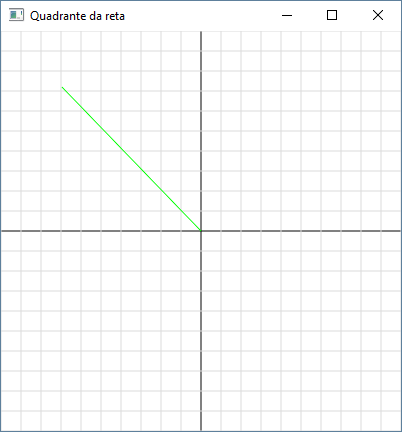
\includegraphics[width=.9\textwidth]{img/cap1_ex4b}}
        \caption{Reta pertencente ao segundo quadrante}
        \label{fig:cap01_ex4b}
    \end{subfigure}
    ~
    \begin{subfigure}{0.2\textwidth}
        \centerline{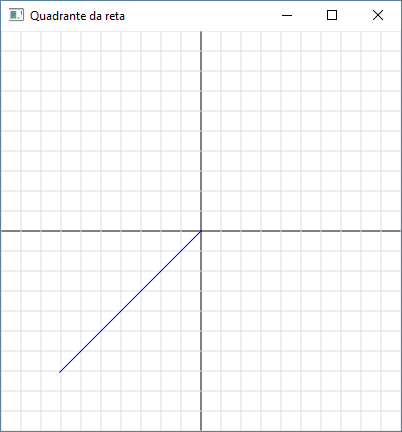
\includegraphics[width=.9\textwidth]{img/cap1_ex4c}}
        \caption{Reta pertencente ao terceiro quadrante}
        \label{fig:cap01_ex4c}
    \end{subfigure}
    ~
    \begin{subfigure}{0.2\textwidth}
        \centerline{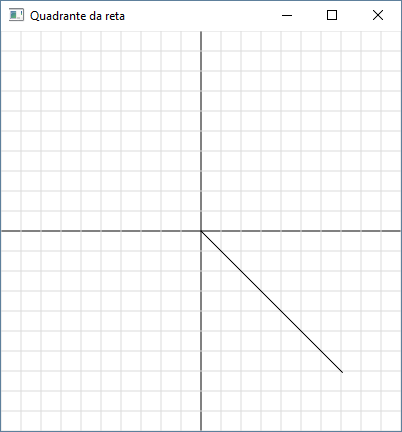
\includegraphics[width=.9\textwidth]{img/cap1_ex4d}}
        \caption{Reta pertencente ao quarto quadrante}
        \label{fig:cap01_ex4d}
    \end{subfigure}

\end{figure*}

\item

Escreva um programa em C que solicita três pontos A, B e C ao usuário, e verifica se esses valores satisfazem a condição de existência do triângulo. Caso essa condição seja satisfeita, exiba esse triângulo e escreva no título da janela se o triângulo é equilátero, isósceles ou escaleno [dica: não usar a função CriaTriangulo()].

  \begin{figure*}[h!]
    \centering
    \begin{subfigure}[b]{0.3\textwidth}
        \centerline{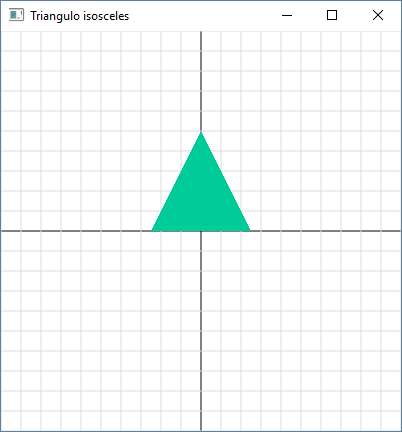
\includegraphics[width=.9\textwidth]{img/cap1_ex23}}
        \caption{Triângulo isósceles}
        \label{fig:cap01_ex23a}
    \end{subfigure}
    ~
    \begin{subfigure}[b]{0.3\textwidth}
        \centerline{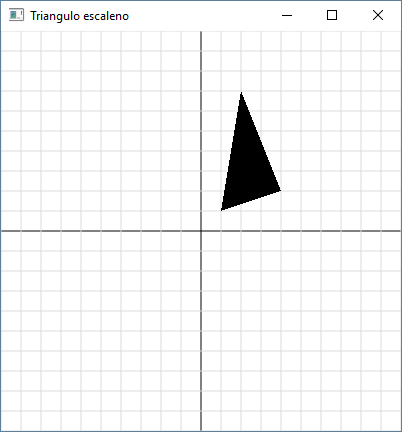
\includegraphics[width=.9\textwidth]{img/cap1_ex23b}}
        \caption{Triângulo escaleno}
        \label{fig:cap01_ex23b}
    \end{subfigure}
    ~
    \begin{subfigure}[b]{0.3\textwidth}
        \centerline{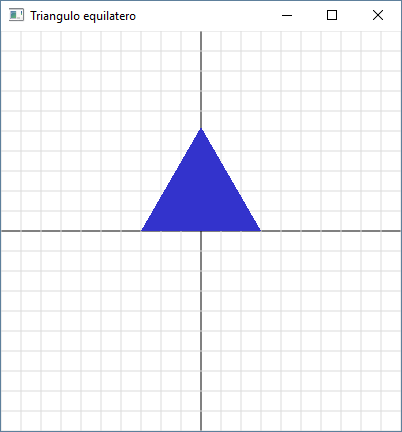
\includegraphics[width=.9\textwidth]{img/cap1_ex23c}}
        \caption{Triângulo equilátero}
        \label{fig:cap01_ex23c}
    \end{subfigure}

\end{figure*}

\label{ex:cap01_ex23}

\end{enumerate}

\section*{Soluções}

\subsection*{Exercício \ref{ex:cap01_ex22}}

Esta prática exibe uma circunferência e indica se dado um ponto qualquer, se este ponto está dentro ou fora da circunferência, exercitando o conceito de distância entre dois pontos. Para a ampliação da espessura do ponto, para ele não ser apenas um pixel, utiliza-se a função \emph{Grafite}.

\lstinputlisting[caption=Código fonte do ponto dentro ou fora da circunferência, style=customc, label=lst:cap1_ex22]{src/ex22_inout.cpp}

\begin{lstlisting}[label={func:CriaReta},language=C++]
int CriaPonto(Ponto p)
\end{lstlisting}
A função \emph{CriaPonto}, na linha \ref{line:CriaPonto}, cria uma geometria do tipo \emph{PONTO}, retornando um índice deste tipo de geometria. Seu único argumento é uma variável do tipo Ponto. Uma geometria do tipo \emph{PONTO} é renderizada como um pixel.

\begin{lstlisting}[label={func:Grafite},language=C++]
void Grafite ( int espessura )
\end{lstlisting}
A função Grafite, na linha \ref{line:Grafite}, aumenta as linhas de rasterização da última geometria criada, variando de $1$ a $\infty$. Por padrão, todas as geometrias começam com esta linha igual a 1. Esta função pode ser usada para deixar mais visível geometrias do tipo PONTO, que possuem 1 pixel de tamanho.

\subsection*{Exercício \ref{ex:cap01_ex4}}
Esta prática exibe uma reta com cor variada de acordo com qual quadrante ela pertence. A função \emph{Pintar} neste caso se refere a única geometria criada no programa, no caso, a reta.
\lstinputlisting[caption=Código fonte do quadrante da reta, style=customc, label=lst:cap1_ex4]{src/ex4_reta.cpp}

\begin{lstlisting}[label={func:CriaReta},language=C++]
int CriaReta(Ponto p1, Ponto p2)
\end{lstlisting}
A função \emph{CriaReta}, na linha \ref{line:CriaReta}, cria uma geometria do tipo \emph{RETA}, retornando um índice deste tipo de geometria. Seu primeiro e segundo argumento são duas variáveis do tipo Ponto.

\subsection*{Exercício \ref{ex:cap01_ex23}}

Esta prática exercita o conceito matemático de condição de existência e de classificação de triângulo, além de exercitar \emph{ifs} aninhados.

\lstinputlisting[caption=Código fonte de exibir triângulo caso ele exista, style=customc, label=lst:cap1_ex23]{src/ex23_exibetriangulo.cpp}
\chapter[Algoritmos com repetição]
{Algoritmos com repetição}



\section*{Resumo}

Estruturas de repetição são criadas para que diversas instruções sejam executadas um determinado número de vezes, enquanto a condição se manter verdadeira.


%\begin{chapreferences}{1.}
%\bibliography{playAPC{}}
%\bibliographystyle{plain}
%\nocite{cbook}
%\nocite{sb6}
%\nocite{glfw}
%\nocite{cppbook}

%\end{chapreferences}

% \begin{chapreferences}{1}

% \bibitem{sb6}
% {\em OpenGL SuperBible}.
% \newblock Pearson Education Inc, 6 edition, 2014.

% \bibitem{glfw}
% Marcus Geelnard and Camilla Berglund.
% \newblock {\em GLFW - Reference guide}, 2010.
% \newblock API version 2.7.

% \bibitem{cbook}
% Brian~W. Kernighan and Dennis~M. Ritchie.
% \newblock {\em The C Programming Language}.
% \newblock 1989.

% \bibitem{cppbook}
% Stanley~B. Lippman, Josés Lajoile, and Barbara Moo.
% \newblock {\em C++ Primer}.
% \newblock 2013.
% \end{chapreferences}

\section*{Pré-requisitos}

As práticas deste capítulo exigem que sejam utilizadas as funções
\begin{itemize}
  \item 
    \begin{lstlisting}[language=C++]
    int CriaGrupo()
    \end{lstlisting}

  \item
    \begin{lstlisting}[language=C++]
    void Move(Ponto p, int grupo)
    \end{lstlisting}

  \item
    \begin{lstlisting}[language=C++]
    int Desenha1Frame()
    \end{lstlisting}

  \item
    \begin{lstlisting}[language=C++]
    void Gira( float theta , int index )
    \end{lstlisting}

  \item
    \begin{lstlisting}[language=C++]
    int ApertouTecla(int tecla)
    \end{lstlisting}

  \item
    \begin{lstlisting}[language=C++]
    int AbreImagem(const char *src)
    \end{lstlisting}

  \item
    \begin{lstlisting}[language=C++]
    void AssociaImagem(int textura, geometrias_validas nome, int index)
    
    \end{lstlisting}
 
\end{itemize}

\section*{Problemas}
\begin{enumerate}

\item
  Exiba um carrinho se movendo de $-100$ à $100$.
  \label{ex:cap01_ex6}

  \begin{figure}[H]
    \centerline{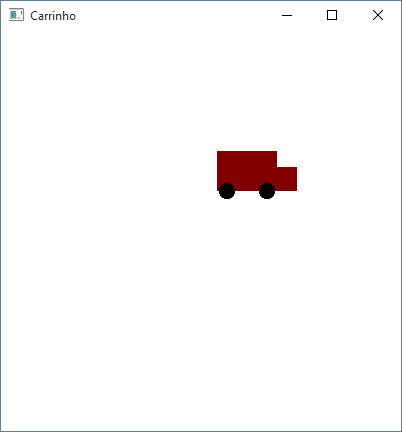
\includegraphics[width=.5\textwidth]{img/cap1_ex5.png}}
    \caption{Carro se movendo da posição -100 até a posição 100}
    \label{fig:cap01_ex6}
  \end{figure}

\item
  Construa um moinho de vento e coloque apenas as hélices para girar.
  \label{ex:cap01_ex7}

  \begin{figure}[H]
    \centerline{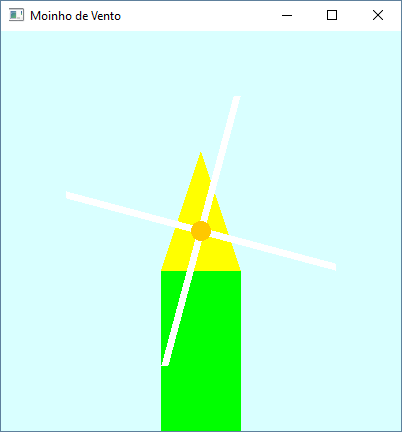
\includegraphics[width=.5\textwidth]{img/cap1_ex7.png}}
    \caption{Moinho de vento}
    \label{fig:cap01_ex7}
  \end{figure}

\item
  Escreva um programa utilizando a playAPC que simula simultaneamente o movimento da Terra ao redor do Sol e o movimento da Lua ao redor da Terra. Considere que as trajetórias de ambas são elípticas. No caso da Terra, o Sol é um dos focos e no caso da Lua, a Terra é um dos focos. Não é necessário simular a proporção real entre os semieixos maiores (a) da Lua e da Terra, nem a excentricidade (e) das duas trajetórias. Encontre empiricamente valores de (a) e (e) de forma que seja possível observar trajetórias elípticas. Simule, porém, a proporção real entre os movimento de translação da Terra e da Lua.
  \label{ex:cap01_ex24}

  \begin{figure}[H]
    \centerline{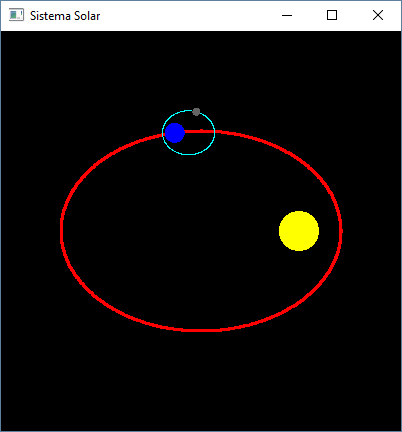
\includegraphics[width=.5\textwidth]{img/cap1_ex24.png}}
    \caption{Sistema solar}
    \label{fig:cap01_ex24}
  \end{figure}

\item
  Sabe-se que a equação da espiral hiperbólica pode ser defina por
\begin{equation} \label{eq:espiral}
  \begin{matrix}
  x	& = &	a \cos(\theta) \\ 
  y	& = &	a \sin(\theta)
  \end{matrix}.
\end{equation}
  onde $a$ é a assíntota para y e $\theta$ o ângulo equivalente ao ângulo em coordenadas polares. Para $a \gets 100$ e $\theta \in (0, 4\pi)$, desenhe duas espirais hiperbólicas calculando seus pontos como é descrito na Equação \ref{eq:espiral}. Para ponto $p$ em $(x,y)$ de uma das hiperbólica, o ponto $p$ da outra espiral deve estar posicionado em $(-x,-y)$.

  \label{ex:cap01_ex5}

  \begin{figure*}[!htp]
    \centering
    \begin{subfigure}[b]{0.3\textwidth}
        \centerline{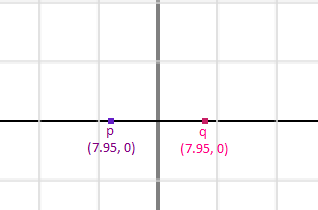
\includegraphics[width=.9\textwidth]{img/cap1_ex6}}
        \caption{Posição inicial aproximada de ambas as espirais}
        \label{fig:cap01_ex6a}
    \end{subfigure}
    ~
    \begin{subfigure}[b]{0.3\textwidth}
        \centerline{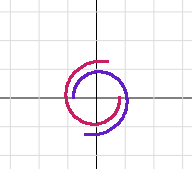
\includegraphics[width=.9\textwidth]{img/cap1_ex6b}}
        \caption{100º iteração no processo de criação das espirais}
        \label{fig:cap01_ex6b}
    \end{subfigure}
    ~
    \begin{subfigure}[b]{0.3\textwidth}
        \centerline{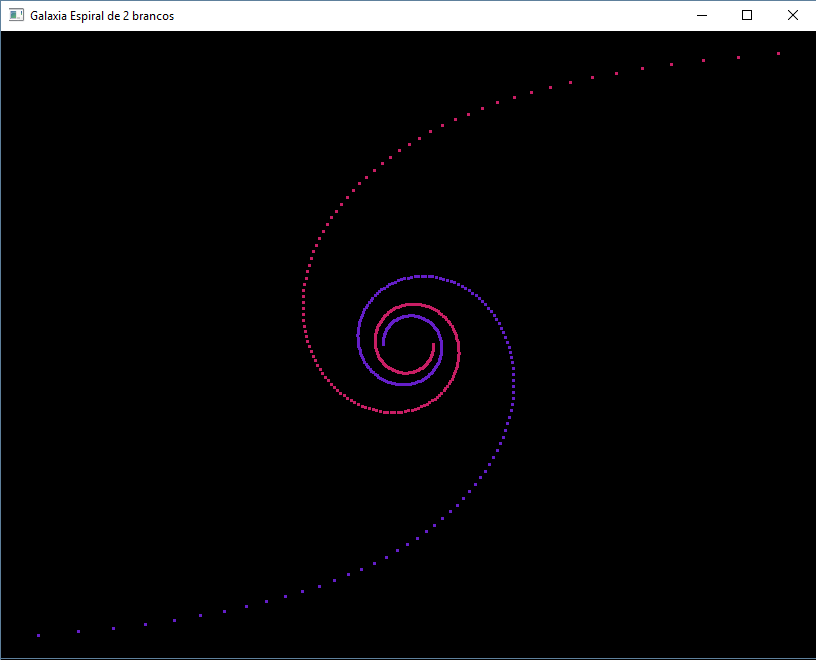
\includegraphics[width=.9\textwidth]{img/cap1_ex6c}}
        \caption{Espiral completa}
        \label{fig:cap01_ex6c}
    \end{subfigure}

\end{figure*}


  \item
  Crie uma animação onde o Mário deve começar no canto esquerdo da tela e seu objetivo é andar até o canto direito da tela. Porém, haverão dois canos que serão posicionados aleatoriamente no meio do caminho, forçando o Mário a pulá-los para não colidir com eles. 
  Para criar a animação de andar, altere as imagens do retângulo onde será desenhado o Mario com a função \emph{AssociaImagem} e, após essa chamada, utilize a função \emph{Desenha1Frame} para renderizar a troca de imagens.

  Para simplificação do problema, considere que o Mário, ao realizar o pulo, ele deva executar meia trajetória circular, onde $\theta$ varia de $\pi$ até $0$ e o raio do pulo seja de $40$ unidades.
  \label{ex:cap01_ex25}

  \begin{figure*}[!htp]
    \centering
    \begin{subfigure}[b]{0.3\textwidth}
        \centerline{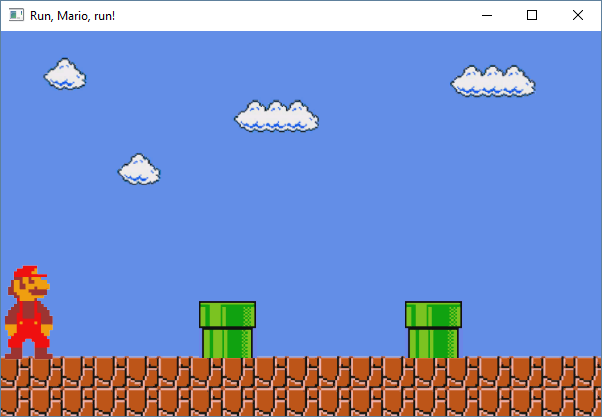
\includegraphics[width=.9\textwidth]{img/cap1_ex25}}
        \caption{Começo da animação}
        \label{fig:cap01_ex6a}
    \end{subfigure}
    ~
    \begin{subfigure}[b]{0.3\textwidth}
        \centerline{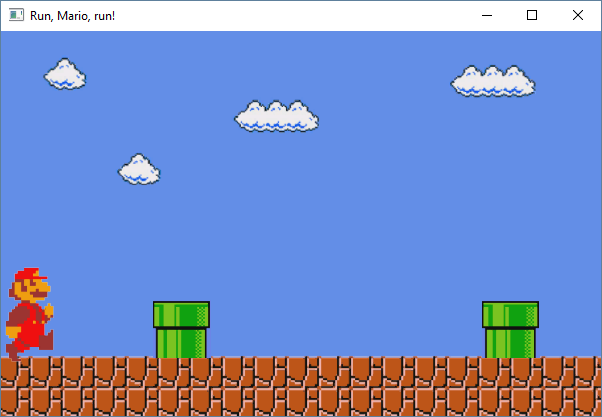
\includegraphics[width=.9\textwidth]{img/cap1_ex25b}}
        \caption{Parte 1 da animação do Mário}
        \label{fig:cap01_ex6b}
    \end{subfigure}
    ~
    \begin{subfigure}[b]{0.3\textwidth}
        \centerline{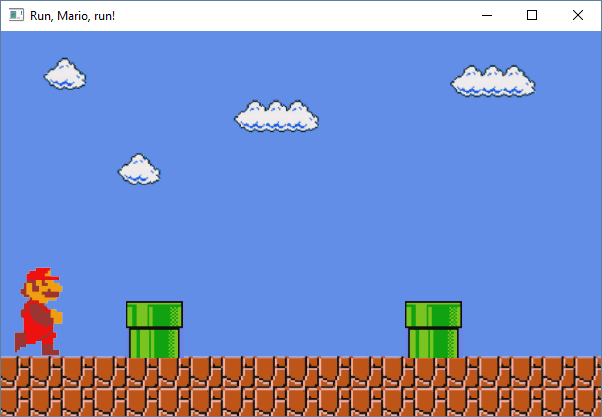
\includegraphics[width=.9\textwidth]{img/cap1_ex25c}}
        \caption{Parte 2 da animação do Mário}
        \label{fig:cap01_ex6c}
    \end{subfigure}
    ~
    \begin{subfigure}[b]{0.3\textwidth}
        \centerline{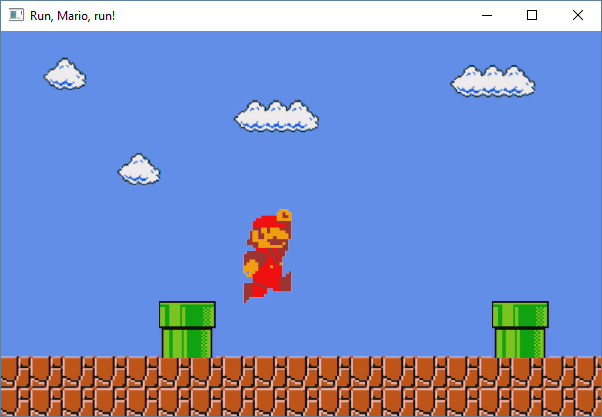
\includegraphics[width=.9\textwidth]{img/cap1_ex25d}}
        \caption{Mário pulando}
        \label{fig:cap01_ex6c}
    \end{subfigure}

  \end{figure*}

\end{enumerate}

\section*{Soluções}

\subsection*{Exercício \ref{ex:cap01_ex6}}

Esta prática exibe um carro construído com dois retângulos e dois círculos, agrupados com a função \emph{CriaGrupo}, movendo-se da posição -100 até a posição 100. Nota-se que todas as geometrias que estão abaixo da função \emph{CriaGrupo} pertencem a um único grupo, o grupo \emph{carro}.
\lstinputlisting[caption=Código fonte do carro andando, style=customc, label=lst:cap1_ex6]{src/ex5_carrinho.cpp}

\begin{lstlisting}[label={func:CriaGrupo},language=C++]
int CriaGrupo()
\end{lstlisting}
A função \emph{CriaGrupo}, na linha \ref{line:CriaGrupo}, agrupará todo um conjunto de geometrias, associando todas a uma única variável, em um único conjunto. Desta forma, é possível transformar um conjunto de geometrias de forma independente, apenas referenciando a variável do grupo.

\begin{lstlisting}[label={func:Move},language=C++]
void Move(Ponto p)
void Move(Ponto p, int index)
\end{lstlisting}
A função \emph{Move}, na linha \ref{line:Movem1}, é uma das três funções de transformação implementadas na \playAPC{}. Há duas formas de utilizar esta função. No caso da Listagem \ref{lst:cap1_ex6}, seu primeiro argumento é o ponto no plano cartesiano que se deseja mover toda as geometrias e o segundo argumento o grupo que se deseja mover. O grupo será transladado até que o ponto de referência da primeira geometria deste grupo esteja no novo ponto desejado, utilizando a Definição \ref{def:translacao}.

\begin{myDef} 
Seja $x$ a coordenada do eixo x original do ponto, $y$ a coordenada do eixo y original do ponto, $x'$ a coordenada resultado do eixo x e $y'$ a coordenada resultante do eixo y.
$$
  \begin{matrix}
  x' = x + d_{x} &\\
  y' = y + d_{y}
  \end{matrix}
$$
Onde $d_{x}$ e $d_{y}$ são o incremento dada a posição original do ponto.
\label{def:translacao}
\end{myDef}

\begin{lstlisting}[label={func:Desenha1Frame},language=C++]
int Desenha1Frame()
\end{lstlisting}
A função \emph{Desenha1Frame}, na linha \ref{line:Desenha1Frame}, renderiza pelo menos $\frac{1}{60}$ segundos da cena, possuindo um controle de 60 frames por segundo. Caso o usuário feche a janela ou aperte a tecla ESC, esta função retornará 0 e encerrará o processo de renderização. Caso contrário, retornará 1.

\subsection*{Exercício \ref{ex:cap01_ex7}}

Esta prática exibe um moinho de vento criado com um grupo composto por um triângulo e um retângulo, o grupo \emph{moinho}, e outro grupo composto pelas hélices, o grupo \emph{helices}. Somente o \emph{helices} sofre a ação de girar. 
\lstinputlisting[caption=Código fonte do moinho, style=customc, label=lst:cap1_ex7]{src/ex7_moinho.cpp}

\begin{lstlisting}[label={func:Gira},language=C++]
void Gira(float theta)
void Gira(float theta, int index)
\end{lstlisting}
A função \emph{Gira}, na linha \ref{line:Giram1}, é uma das três funções de transformação implementadas na \playAPC{}. Há duas formas de utilizar esta função. No caso da Listagem \ref{lst:cap1_ex7}, seu primeiro argumento é um ângulo $\theta$ em graus e seu segundo argumento indica o grupo que irá sofrer a ação de girar, recalculando a posição de cada pixel utilizando a Definição \ref{def:rotacao}. 

\begin{myDef} 
Seja $x$ a coordenada do eixo x original do ponto, $y$ a coordenada do eixo y original do ponto, $x'$ a coordenada resultado do eixo, $y'$ a coordenada resultante do eixo y e $\theta$ o ângulo em graus de rotação.
$$
  \begin{matrix}
  x' = x\cos \theta  - y \sin \theta &\\
  y' = x\sin \theta  + y \cos \theta
  \end{matrix}
$$
\label{def:rotacao}
\end{myDef}


\subsection*{Exercício \ref{ex:cap01_ex5}}

Esta prática ilustra como a função \emph{Desenha1Frame} pode ser utilizada. Na linha \ref{line:ex6_for} até a linha \ref{line:ex6_forend}, a cada iteração são criados dois pontos, um de cada espiral.
\lstinputlisting[caption=Código fonte da galáxia expiral, style=customc, label=lst:cap1_ex5]{src/ex6_galaxy.cpp}

\begin{lstlisting}[label={func:Gira},language=C++]
void Gira(float theta)
void Gira(float theta, int index)
\end{lstlisting}
A função \emph{Gira}, na linha \ref{line:Giram2}, é uma das três funções de transformação implementadas na \playAPC{}. Há duas formas de utilizar esta função. No caso da Listagem \ref{lst:cap1_ex5}, seu primeiro argumento é um ângulo $\theta$ em graus e ele irá girar todas as geometrias criadas de acordo com a Definição \ref{def:rotacao}. 


\begin{lstlisting}[label={func:ApertouTecla},language=C++]
int ApertouTecla(int tecla)
\end{lstlisting}
A função \emph{ApertouTecla}, na linha \ref{line:ApertouTecla}, verifica se o usuário pressionou a tecla \emph{tecla} naquela cena. Seu único argumento pode variar de acordo com a Tabela \ref{tab:teclas}.

~\begin{table}[H]
  \caption{Teclas reconhecidas pela \playAPC{}}
  \centering
    \begin{tabular}{lc}
    \hline
    Valor&\bf Descrição \\
    \hline
    GLFW\_KEY\_$n$  & Teclas alfanuméricas ($n \in (0..9)$ ou $n \in (A..Z)$)  \\
    GLFW\_KEY\_SPACE  & Espaço \\
    GLFW\_KEY\_ESC  & Escape \\
    GLFW\_KEY\_F$n$  & Function key ($n \in (0..25)$) \\
    GLFW\_KEY\_LEFT  & Seta para esquerda \\
    GLFW\_KEY\_UP  & Seta para cima \\
    GLFW\_KEY\_DOWN  & Seta para baixo \\
    GLFW\_KEY\_RIGHT  & Seta para direita \\
    GLFW\_KEY\_LCONTROL  & Control esquerdo \\
    GLFW\_KEY\_RCONTROL  & Control direito \\
    GLFW\_KEY\_LALT  & Alt esquerdo \\
    GLFW\_KEY\_RALT  & Alt direito \\
    GLFW\_KEY\_TAB  & Tabulador \\
    GLFW\_KEY\_ENTER  & Enter \\
    GLFW\_KEY\_BACKSPACE  & Backspace \\
    GLFW\_KEY\_INSERT  & Insert \\
    GLFW\_KEY\_DEL  & Delete \\
    GLFW\_KEY\_PAGEUP  & Page up \\
    GLFW\_KEY\_PAGEDOWN  & Page down \\
    GLFW\_KEY\_HOME  & Home \\
    GLFW\_KEY\_END  & End \\
    GLFW\_KEY\_KP\_$n$  & Teclas numéricas do keypad ($n \in (0..9)$)\\
    GLFW\_KEY\_KP\_DIVIDE  & Tecla dividir do keypad ( \div )\\
    GLFW\_KEY\_KP\_MULTIPLY  & Tecla multiplicar do keypad ( \times )\\
    GLFW\_KEY\_KP\_SUBTRACT  & Tecla subtrair do keypad ( - )\\
    GLFW\_KEY\_KP\_ADD  & Tecla adição do keypad ( + )\\
    GLFW\_KEY\_KP\_EQUAL  & Tecla igual do keypad ( = )\\
    GLFW\_KEY\_KP\_NUMLOCK  & Tecla Numlock do keypad ( = )\\
    GLFW\_KEY\_CAPS\_LOCK  & Caps lock\\
    GLFW\_KEY\_SCROLL\_LOCK  & Scroll lock\\
    GLFW\_KEY\_PAUSE  & Pause\\
    GLFW\_KEY\_MENU  & Menu\\
    \hline
  \end{tabular}
  \label{tab:teclas}
\end{table}

\subsection*{Exercício \ref{ex:cap01_ex25}}
Esta prática introduz o conceito de colisão de objetos, com uma colisão entre dois retângulos, e também ao uso de imagens. Na introdução a utilização de imagens, não é necessário que o aluno tenha como pré-requisito o conceito de manipulação de arquivos em C. Como a função \emph{Desenha1Frame} renderiza $\frac{1}{60}$ segundos, para criar o efeito de uma animação menos fluída, se faz necessário sua chamada repetidas vezes.

\lstinputlisting[caption=Código fonte do Mario animado, style=customc, label=lst:cap1_ex25]{src/ex25_mario.cpp}

\begin{lstlisting}[label={func:AbreImagem},language=C++]
int AbreImagem(const char *src)
\end{lstlisting}
A função \emph{AbreImagem}, na linha \ref{line:AbreImagem}, recebe como argumento o caminho, relativo ou absoluto, da imagem que se deseja carregar no programa. Ela retorna um índice associado àquela imagem, que deve ser passado como argumento para a função \emph{AssociaImagem}. A função \emph{AbreImagem} consegue ler imagens de extensão \emph{bmp}, \emph{jpg} e \emph{png}.

\begin{lstlisting}[label={func:AssociaImagem},language=C++]
void AssociaImagem(int textura)
void AssociaImagem(int textura, geometrias_validas nome, int index)
\end{lstlisting}
A função \emph{AssociaImagem}, na linha \ref{line:AssociaImagemm1}, possui duas formas de ser utilizada. No caso da Listagem \ref{lst:cap1_ex25}, ele associa a imagem a última geometria que foi definida, no caso, o retângulo do background. Para criar o efeito de animação no Mario, determinou-se que o retângulo Mario seria a última geometria do último grupo criado. Dessa forma, as próximas chamadas da função \emph{AssociaImagem} estariam referenciando o retângulo da linha \ref{line:ultimoRetangulo}.

